\section{Van der Pol Oscillator}
\label{Van der Pol Oscillator}


Applying the UKF to the Van der Pol oscillator will be used as a simple example to demonstrate the impacts of measurement and process noise. The Van der Pol equation, so named after its developer Balthasar Van der Pol, describes a self sustaining oscillator that create energy at small amplitudes and remove energy from large amplitudes. The Van der Pol equation describes a nonconservative oscillator (also known as a relaxation oscillator). Applications of the Van der Pol oscillators include circuits, vacuums, and modeling biological systems
 \cite{weisstein_2019}. The Van der Pol oscillator is represented by a nonlinear second order differential equation: 
\begin{align*}
\frac{d^2y}{dt^2} + \mu(y^2-1)\frac{dy}{dt} = 0
\end{align*}   \\
where $\mu$ is a damping coefficient, $\frac{d^2y}{dt^2}$ is acceleration, $\frac{dy}{dt}$ is velocity, and $y$ is position. Therefore, for all $\mu < 0$, dampening occurs and the system tends to 0. The rate at which the system converges to zero is dependent on the size of $\mu$, with larger values taking longer to converge and smaller values converging faster. If $\mu = 0$, the system becomes a simple harmonic oscillator, where motion is periodic. Lastly, if $\mu > 0$, the system enters a limit cycle, which is an isolated closed trajectory. \cite{kinoshita_2013}. \\ 

\noindent The UKF can be applied to this nonlinear system to determine where the system will be at a point in time. To do so, relevant state variables include position and velocity. 
\begin{align*}
x_k = \begin{bmatrix}
          y\\ 
          v
           \end{bmatrix}  
\end{align*}


\noindent Transforming the Van der Pol equation from a second order differential equation to a first order differential equation makes it easier to define $f$, the state function of the system. By substituting $v$ for $\frac{dy}{dt}$, and $ \frac{dv}{dt} $ for  $\frac{d^2y}{dt^2}$ one can rewrite the Van der Pol equation as 
  \begin{align*}
 	\frac{dv}{dt}  +\mu(y ^2-1)v + y = 0.
 \end{align*}

\noindent From this, we get the differential equations associated with the state variables to generate the nonlinear transformation function $f$. For the sake of simplicity, assuming $\mu = 1$, we get
\begin{align*}
\dot x_k  = 
	\begin{bmatrix}
           \frac{dy}{dt}  \\ \\
           \frac{d^2y}{dt^2} 
           \end{bmatrix} = 
           \begin{bmatrix}
          v \\ \\
           \frac{dv}{dt} 
           \end{bmatrix}  =
           \begin{bmatrix}
           v \\ \\
           -1 (y^2 - 1)v - y 
           \end{bmatrix}=
           \begin{bmatrix}
           0 & 1 \\ \\
           -1& 1- y^2 
           \end{bmatrix} x_k 
           =
           f.
\end{align*}


\noindent In this particular example, the only measurement received from the system is position. Therefore, this filter is continually correcting for the position state state variable through measurement function $h$. Here, measurements of the system are simulated by adding noise to the position state variable. Even though there are only measurements for one state variable, we can still generate estimates of both state variables. In terms of hyper-parameters $\alpha, \kappa$, and $\beta$, default values were used.\\ 

\noindent To simulate a Van der Pol Oscillator, an ordinary differential equation solver can be applied to state function $f$ to generate true values of the system. Simulating data was done by adding noise to the system, such that the noise was normally distributed with a mean of 0 and variance of $R$. All of the code used to simulate the UKF for the Van der Pol oscillator is from \cite{matlab_simulink}. \\

\noindent The results of the UKF on the Van der Pol oscillator are given in Figure ~\ref{fig:VDP}. The top graph is for position, which is why there are measured values, and the bottom graph is for velocity. For the position graph, there is a large variation in measurements, but the UKF is able to correct the prediction such that it converges with the true values and not the measured values. In both states, the UKF estimate is able to quickly converge to the system's true values. This is because the model is initialized with values close to the true system values and because levels of process noise and measurement noise is low.  \\

\noindent The second state variable has strong performance despite not being corrected for because the ODE for velocity is dependent on position. Therefore, by correcting for position, velocity is also being corrected. However, in the case where only velocity is being corrected for, it is expected that the UKF will perform strongly for the velocity state variable and poorly for the position state variable.


\comment{
\noindent All of this can be modeled on Matlab; all source code is from Matlab and can be referenced in Appendix A \cite{matlab /& simulink}
}

\begin{figure}[ht]
    \centering
    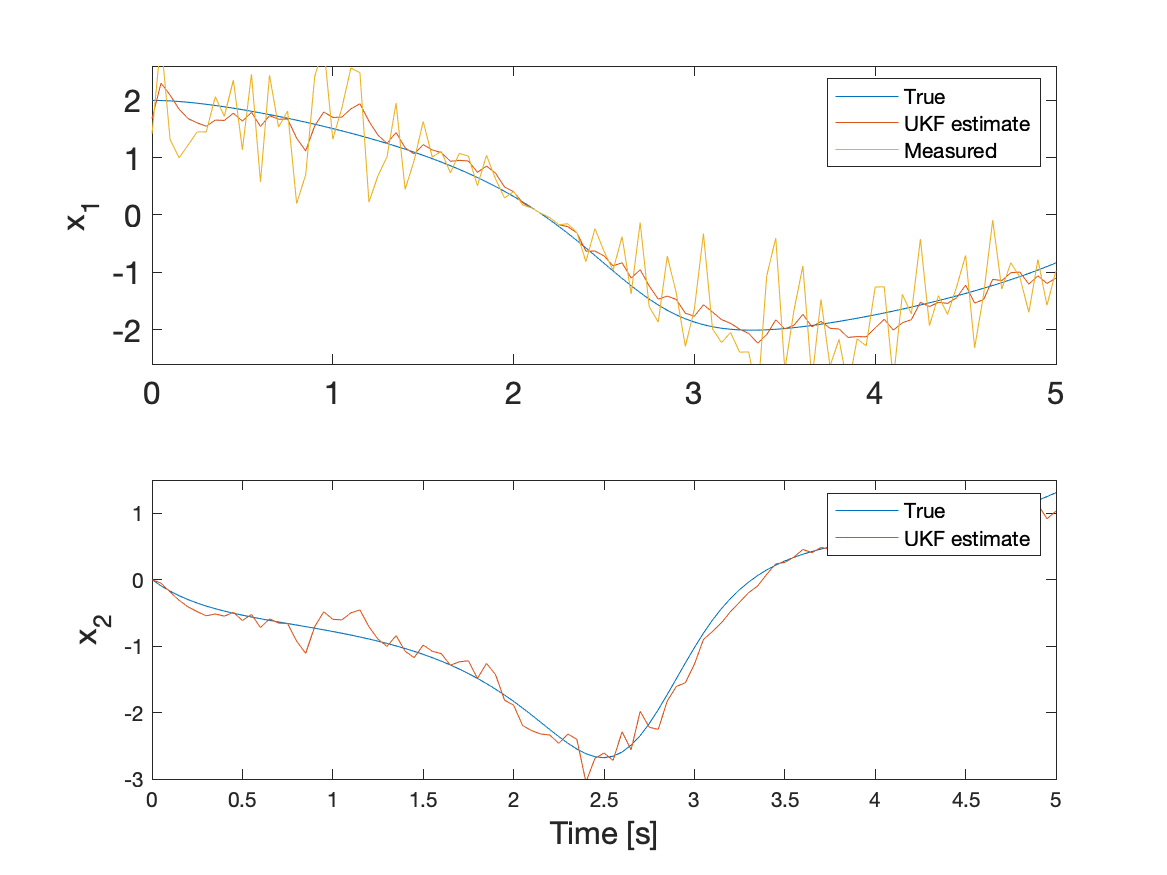
\includegraphics[scale = 0.6]{VDP.png}
    \caption{The top graph is represents position and the bottom graph represent velocity. In both cases, the UKF model has parameters R = 0.2, Q = diag[0.02, 0.1], and the initial state is $x_0=$[2,0], which is the true initial value.
    As expected, the model converges with the true values of the system for both state variables. In this case, the only measurements we are receiving from the system are position, which is why the second state variable has no measured values.}
\label{fig:VDP}
\end{figure}

\clearpage

\noindent In the real world, it cannot be assumed that all models will be initialized with the system's true initial values. Figure ~\ref{fig:BADVDP} illustrates UKF performance, given the same parameters of Figure ~\ref{fig:VDP}, except for an initial value of $x_0=$[1, 7]  instead of $x_0=$[2,0]. The initial value of $x_0=$[1, 7]  is chosen arbitrarily. As expected, initial values that are further from the system's true initial values cause convergence to take place at a slower rate. Since position's initial state was closer to the true value as compared to velocity's initial state, the position state variable converged faster. Another factor for position's quicker convergence is the fact that it is the state being corrected for. Velocity, on the other hand, takes awhile to converge, but eventually does after about 1 second. 



\begin{figure}[ht]
    \centering
    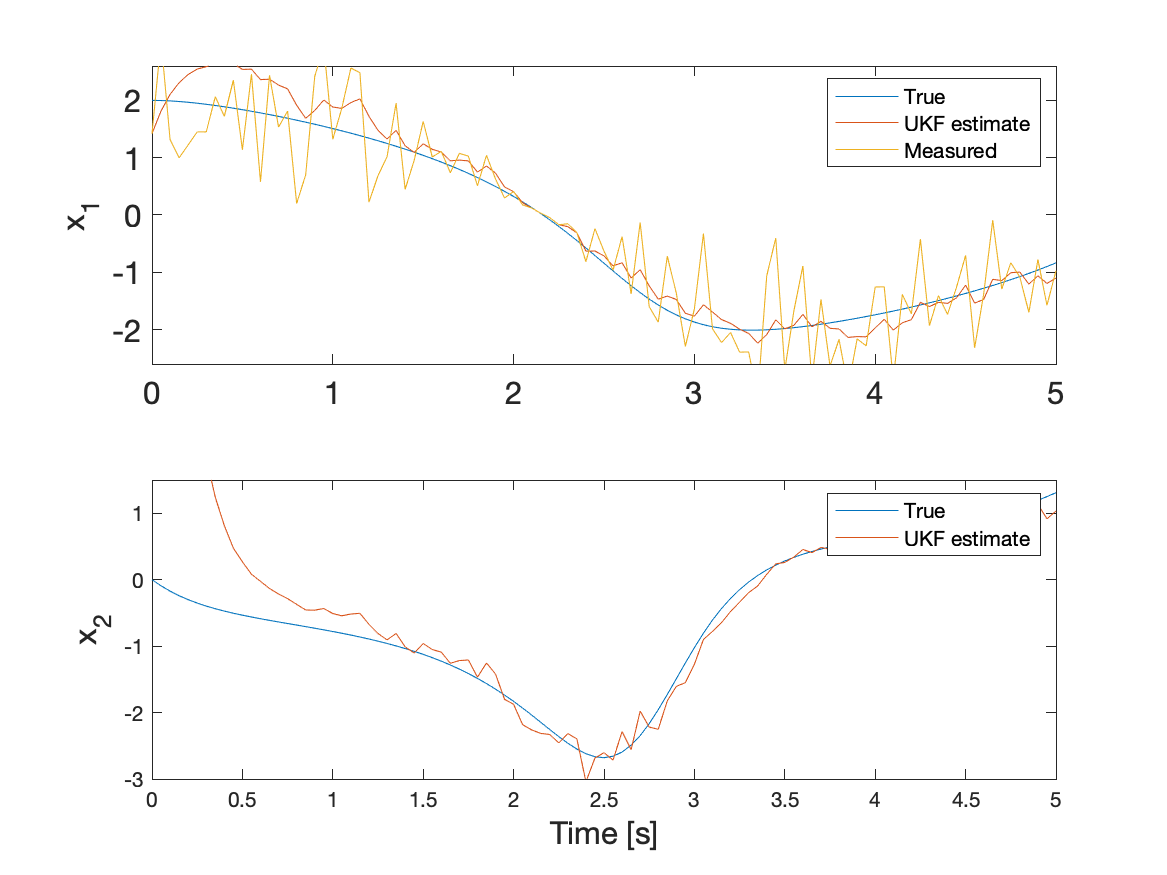
\includegraphics[scale = 0.6]{VDP_badinitial.png}
    \caption{This figure visualizes the performance of the UKF with poor initial conditions: $x_0=$[1, 7]  instead of $x_0=$[2,0]. Inaccurate initial conditions cause convergence to take place more slowly. This seems to be the case, especially in the state variable that is not being corrected for.}
    \label{fig:BADVDP}
\end{figure}

\clearpage

\noindent Figures ~\ref{fig:f1} and ~\ref{fig:f2} demonstrates how measurement noise impacts model convergence. Figure ~\ref{fig:f1} depicts the UKF model with $R=0.9$. This results in variation in the measurements, as visualized through the yellow lines. In terms of model accuracy, there is some fluctuation but for the most part the UKF seems to perform well and converge with the system's true values. Figure ~\ref{fig:f2} depicts the UKF model with $R=0.002$, which was chosen arbitrarily. Here, there is little variation in the measurements. Therefore, the model converges almost instantly with the true values for both state variable.  


\begin{figure}[ht]
  \centering
  \subfloat[UKF with high measurement noise (0.9)]{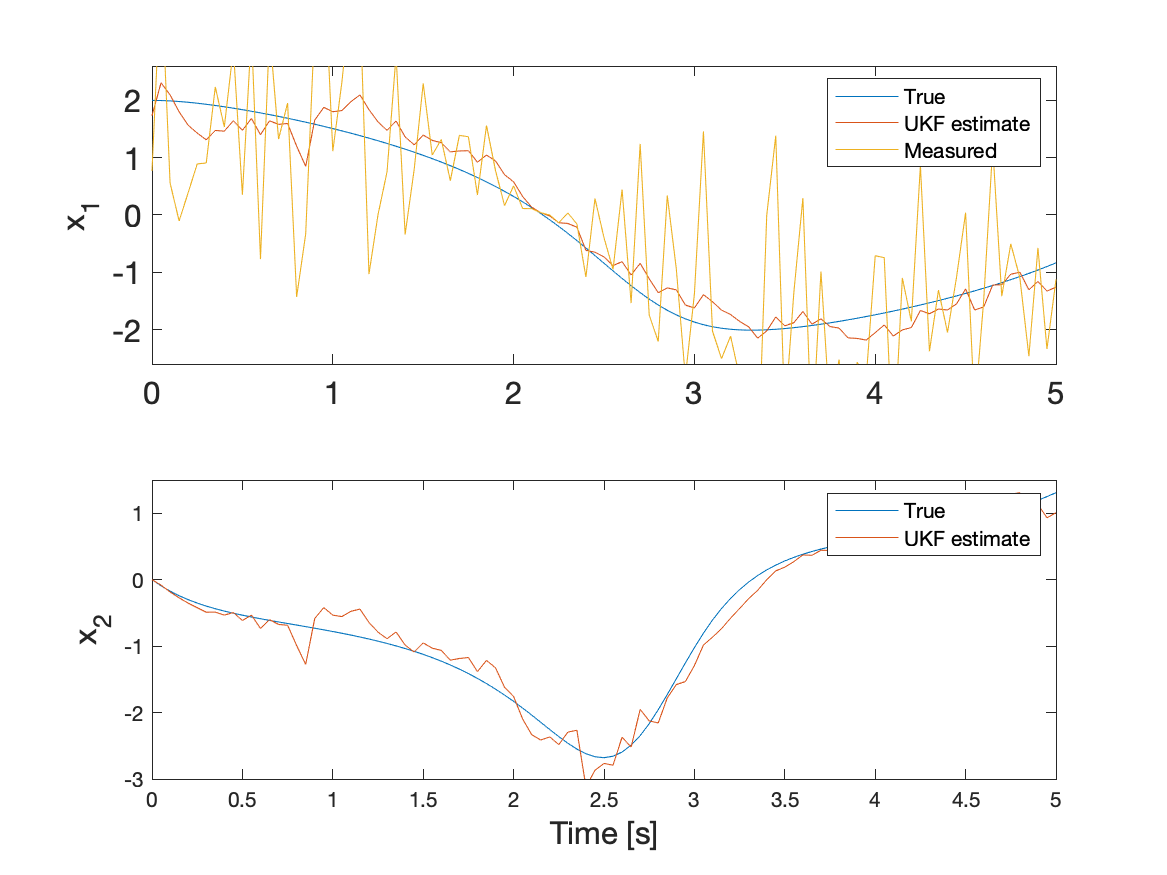
\includegraphics[width=0.55\textwidth]{VDP_highMN.png} \label{fig:f1}}
  \hfill
  \subfloat[UKF with low measurement noise (0.002)]{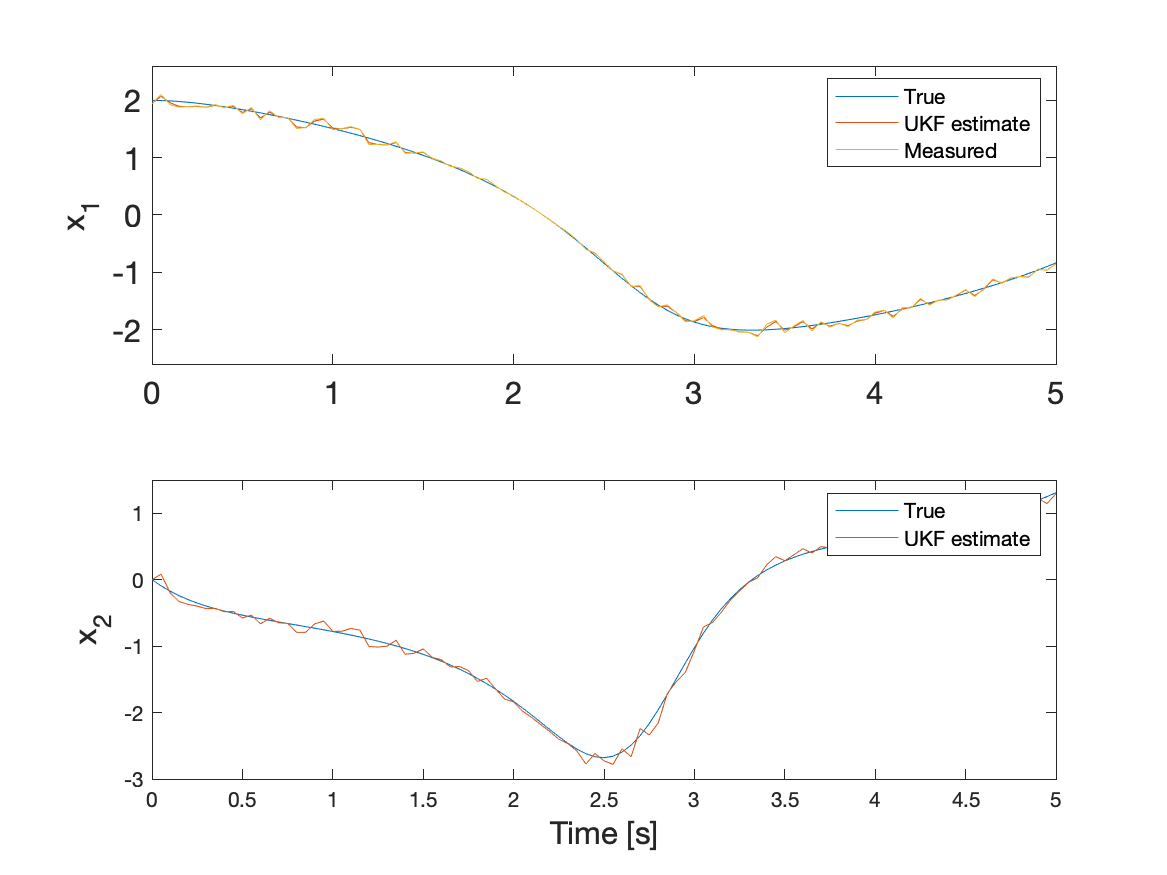
\includegraphics[width=0.55\textwidth]{VDP_lowMN.png} \label{fig:f2}}
  \caption{UKF performance on the VDP oscillator with difference values of measurement noise.
  The model's behavior changes in response to the different values of measurement noise. Even when measurement noise is high, the UKF continues to perform well. Though, the rate of convergence appears to be slower.
On the other hand, when measurement noise is low, the UKF seems to converge instantly with the measured values.}
\end{figure}

\clearpage 
\noindent Figures ~\ref{fig:f3} and ~\ref{fig:f4} demonstrates how process noise impacts model convergence. Process noise is the amount of error in the system, as represented in the ODEs of each state. It is expected that high process noise will result in the model depending on incoming system measurements because it has low confidence in the prediction. On the other hand, low process noise should result in low confidence in the measurements, because the model is depending more on the prediction. This is clearly visualized in the results. Figure ~\ref{fig:f3} depicts the UKF model with high process noise, $Q=[0.9, 0.8]$. Here, the position state variable is almost entirely dependent on the measurements. Even in the last time-step, the UKF is remains closer to the measurements as opposed to the true values of the system. Figure ~\ref{fig:f4} depicts the UKF model with low process noise, $Q=[0.0001, 0.0001]$, which was chosen arbitrarily. Both state variables seem to be somewhat influenced by the measurements in the beginning at the 1 second time step, but later on it almost completely disregards the measurements and converges to the true system values. After the 2 second time step, there is a smoothing in the UKF estimate for both state variables.


\begin{figure}[!ht]
  \centering
  \subfloat[UKF with high process noise (0.9 0.8)]{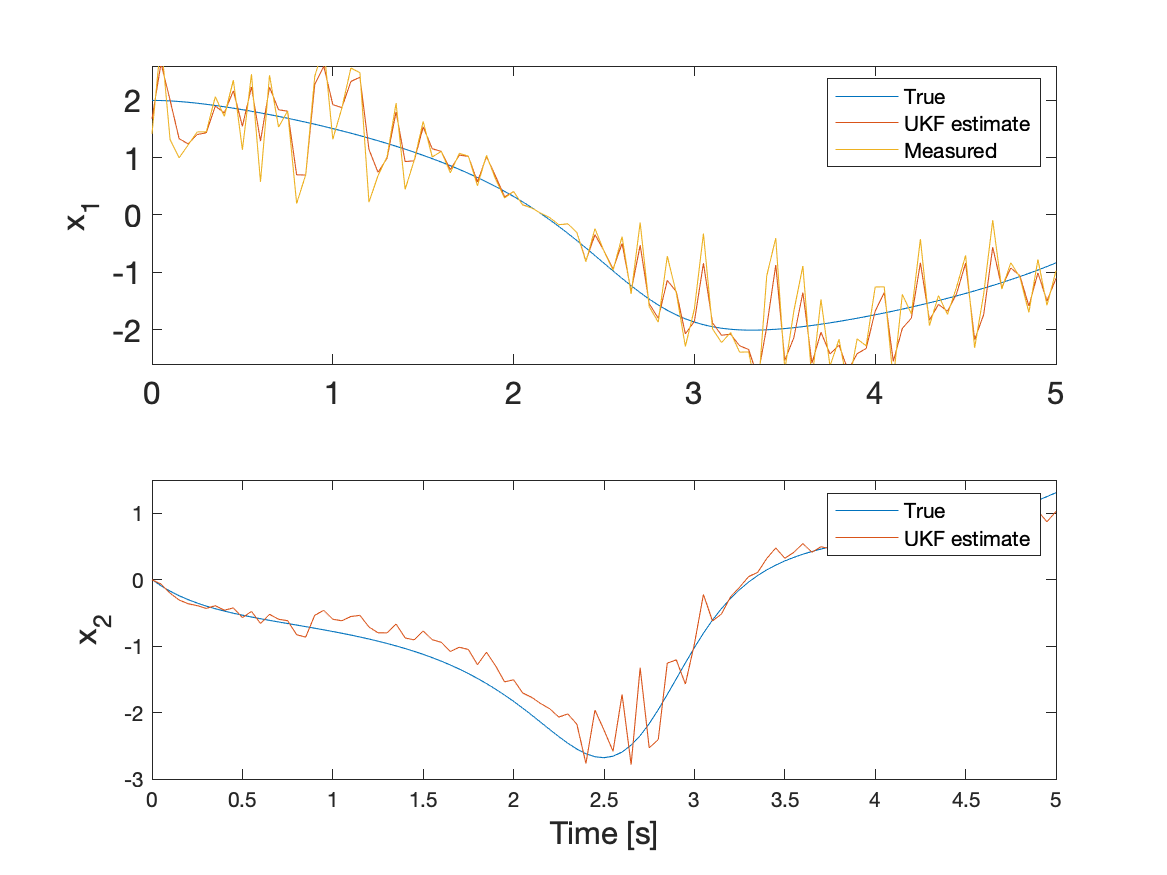
\includegraphics[width=0.5\textwidth]{VDP_highPN.png}\label{fig:f3}}
  \hfill
  \subfloat[UKF with low process noise (0.0001 0.0001)]{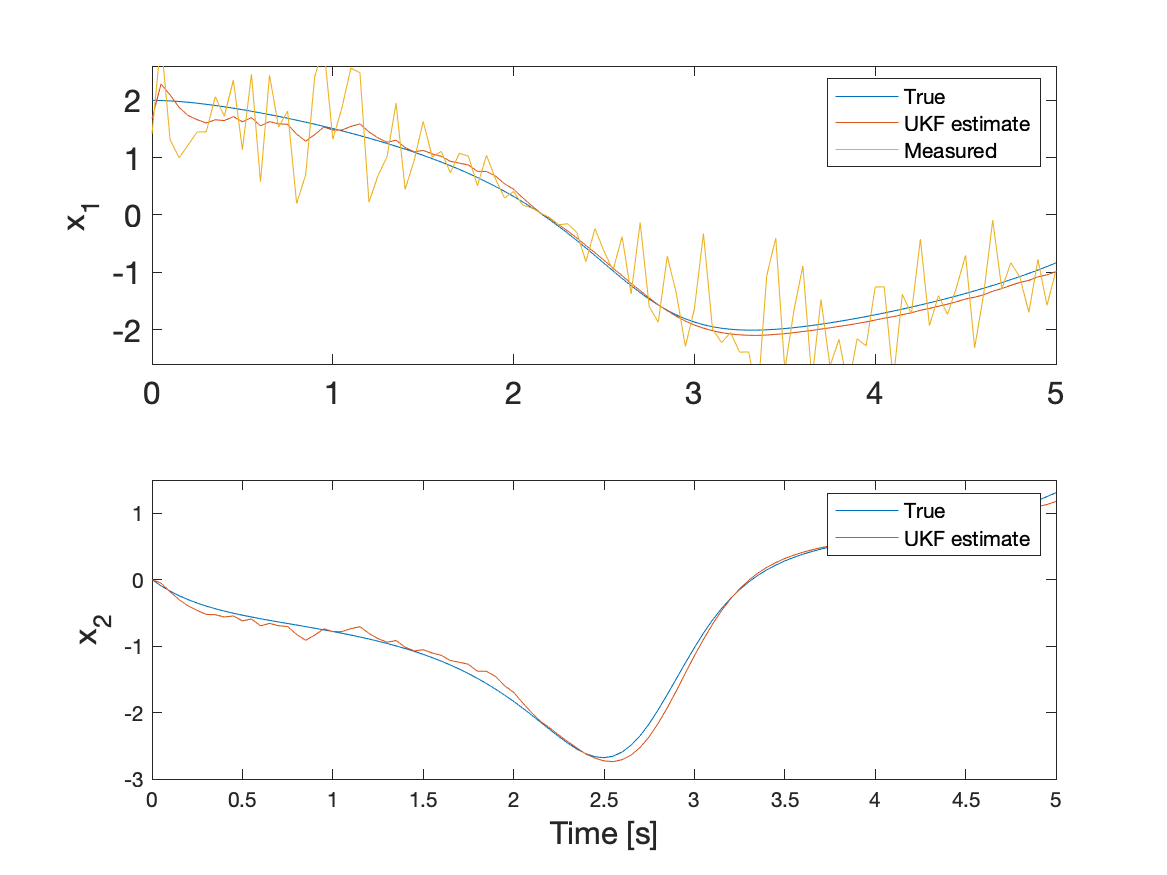
\includegraphics[width=0.5\textwidth]{VDP_lowPN.png}\label{fig:f4}}
  \caption{UKF performance on the VDP oscillator with different values of process noise.
  Recall that process noise measures errors in the model. For the purpose of this example, process error was set to extreme high and low values. In theory, the Van der Pol equation should have small process error because it is a well used equation. Lower process noise seems to have a smoothing effect on the UKF estimate. On the other hand, higher process noise causes the model to almost entirely depend on incoming system measurements.}
  \end{figure}
  
\newpage

\noindent In conclusion, the purpose of this example is to demonstrate how the UKF can be applied to a simple nonlinear system. In addition, this example also explores how the model is impacted by poor initial conditions, measurement noise, and process noise. \\

\noindent Before implementing the UKF, the system must be converted into its discretized state space form. Afterwards, data can be simulated on Matlab by adding Gaussian white noise to the system's true values. In this example, only position was measurable. If only velocity were measurable, the UKF would perform poorly because position is not dependent on velocity. The UKF can be applied to this system, and the performance is quite strong since the model is initiated with values near its true values, measurement noise is small, and process noise is small. \\

\noindent When a model is initiated with values near the system's true values convergence occurs at a faster rate. In the case where the initial conditions is not near the system's true values, convergence can still occur, just at a slower rate. In this example, initializing the model with values further form the truth resulted in the model converging after the 1.5 second time step. Here, the convergence took longer than it did when setting the system to its true values, where convergence took place almost immediately. In the real world, not all models are initialized with the system's true values; therefore, it is important that the UKF is able to correct itself to achieve convergence. \\
   
\noindent Measurement noise, or the amount of variation in the measurements, is another factor that impacts the rate of convergence. By using large measurement noise, there was more variability in the measurements, resulting in convergence to take place slower. The model was initially impacted greatly by noise fluctuation, but eventually converged with its true value. On the other hand, small values of measurement noise caused the model to converge immediately with the system. This is because there is little variability in the measurements, meaning that the measurements are close to the system's true values. Since the measurements are near the true values and process noise is assumed to be small for both cases, the UKF predictions will be almost identical to the system's true values.\\

\noindent Prcoess noise is the amount of error in the system. Low process noise indicates that the UKF will depend less on measurements and more on its prediction. High process noise indicates that the UKF will depend more on measurements and less on the prediction. When applied to the VDP oscillator, one could see how high process noise resulted in the UKF estimate to overlap almost entirely with the measurements. When process noise was low, the system was not influenced too much by noise, and depend more on its prediction, which eventually resulted in a smoothing of the estimate \\

\noindent Tuning performance and model convergence will require an understanding the relationship between initializing a model and the amount of noise in the system. 
   
   
   
   
   
   
    
